\chapter{Simulační výsledky}

\noindent V této kapitole ukážeme výsledky výpočtů Rényiho odhadů na námi generovaných datech. 

Jelikož nám šlo o experimentální ověření robustnosti odhadů, generovali jsme znečištěná data v podobě konvexních směsí znečištěného rozdělení $P$ a znečišťujícího rozdělení $Q$, tedy směsi tvaru $P_\varepsilon(Q) = (1-\varepsilon)P + \varepsilon Q$, pro $\varepsilon \in [0,1]$. V tabulkách i grafech se objevuje 



\begin{figure}[htb]
	\begin{center}
		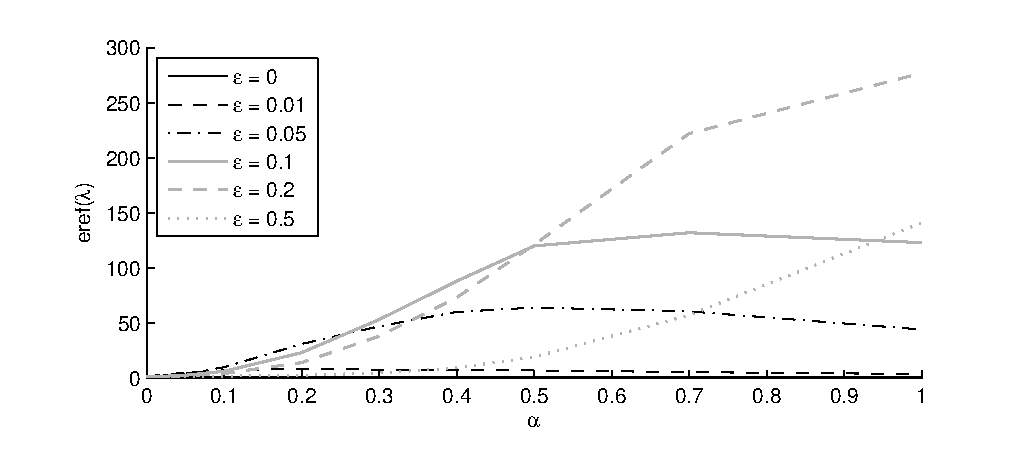
\epsfig{file=Eref-Exp-lambda.eps, height=2.in}
		\caption{Empirická relativní eficience eref($\hat{\lambda}$) minimálního $\mathfrak{R}_\alpha$-odhadu parametru $\lambda$ exponenciálního rozdělení v konvexní směsi 
		$(1-\varepsilon)E(0,1) + \varepsilon E(0,10)$ pro různá znečištění $\varepsilon$.}
		\label{fig-eref-Exp-lambda}
	\end{center}
\end{figure}

\begin{figure}[htb]
	\begin{center}
		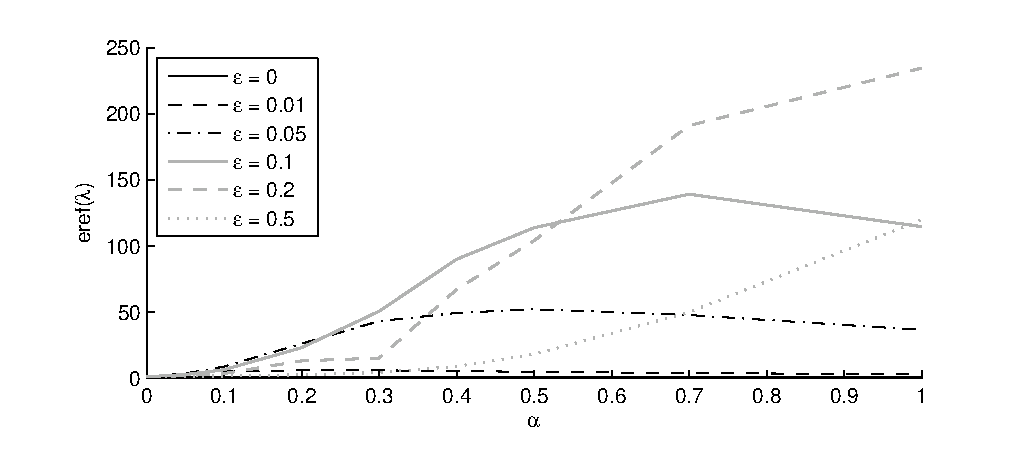
\epsfig{file=Eref-Laplace-lambda.eps, height=2.in}
		\caption{Empirická relativní eficience eref($\hat{\lambda}$) minimálního $\mathfrak{R}_\alpha$-odhadu parametrů  $\mu,\lambda$ Laplaceova rozdělení na datovém souboru o velikosti $n = 500$ generovaném	jako konvexní směs	$(1-\varepsilon)L(0,1) + \varepsilon L(0,10)$ pro různá znečištění $\varepsilon$.}
		\label{fig-eref-Laplace-lambda}
	\end{center}
\end{figure}

\begin{figure}[htb]
	\begin{center}
		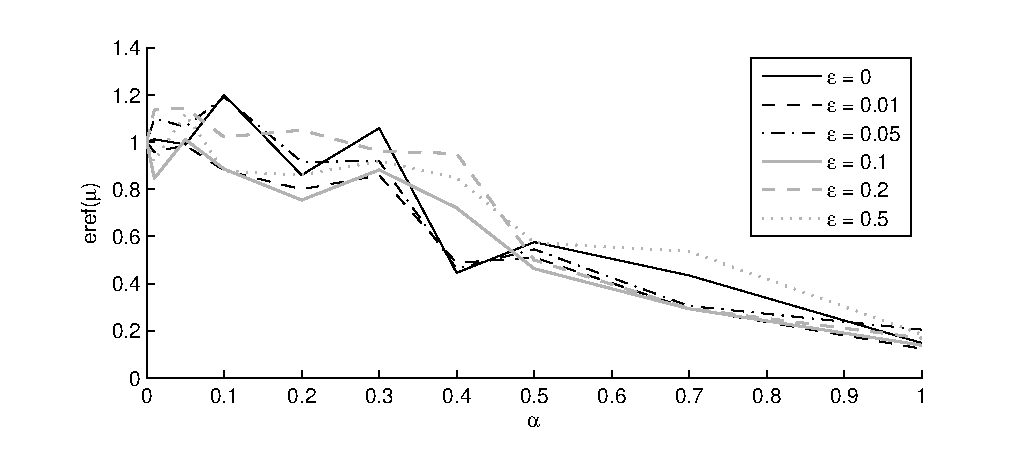
\epsfig{file=Eref-Exp-mu.eps, height=2.in}
		\caption{ TODO }
		\label{fig-eref-Exp-mu}
	\end{center}
\end{figure}

\begin{figure}[htb]
	\begin{center}
		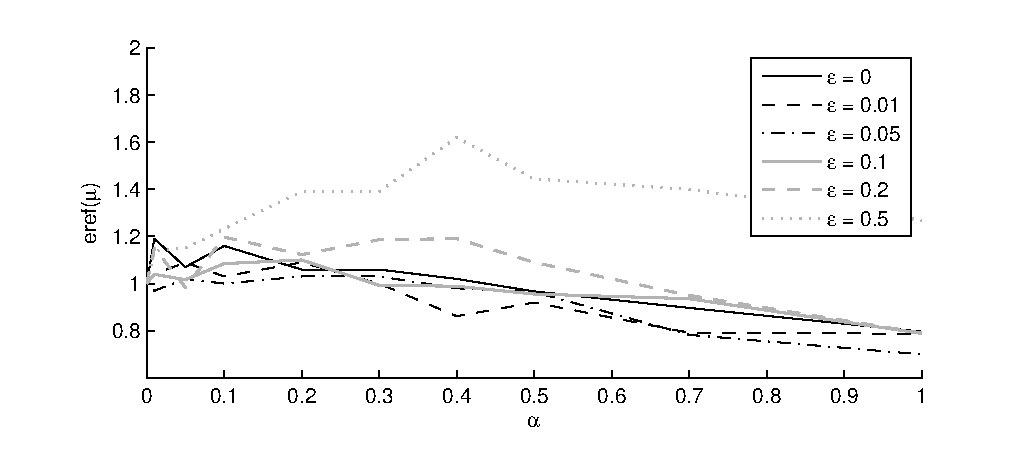
\epsfig{file=Eref-Laplace-mu.eps, height=2.in}
		\caption{ TODO }
		\label{fig-eref-Laplace-mu}
	\end{center}
\end{figure}

